\RequirePackage{plautopatch}
\documentclass[14pt,aspectratio=169,xcolor=dvipsnames,table,onlytextwidth,dvipdfmx]{beamer}
\usepackage[utf8]{inputenc}
\usepackage{bxdpx-beamer} % dvipdfmxなので必要

\usetheme{Boadilla}
%Beamerフォント設定
\usefonttheme{professionalfonts}
\usepackage[T1]{fontenc}
\usepackage[deluxe,uplatex]{otf} % 日本語多ウェイト化
\usepackage{mlmodern}  % 太いComputer Modern
% MLmodernのバグを修正: cf. https://tex.stackexchange.com/questions/646333/size-of-integral-symbol-in-section-header-with-mlmodern
\DeclareFontFamily{OMX}{mlmex}{}
\DeclareFontShape{OMX}{mlmex}{m}{n}{%
   <->mlmex10%
   }{}
\usepackage{newtxtext} % 数式以外をTXフォントで上書き
% \usepackage[noalphabet,unicode]{pxchfon}
% \setminchofont{KozMinPro-Regular.otf}% 游明朝Regular
% \setboldminchofont{KozMinPro-Bold.otf}% 游明朝Demibold
% \setgothicfont[0]{BIZ-UDGothicR.ttc}% BIZ UDゴシックR
% \setboldgothicfont[0]{BIZ-UDGothicB.ttc}% BIZ UDゴシックB
\renewcommand{\familydefault}{\sfdefault}  % 英文をサンセリフ体に
\renewcommand{\kanjifamilydefault}{\gtdefault}  % 日本語をゴシック体に
\usefonttheme{structurebold} % タイトル部を太字
\setbeamerfont{alerted text}{series=\bfseries} % Alertを太字
\setbeamerfont{section in toc}{series=\mdseries} % 目次は太字にしない
\setbeamerfont{frametitle}{size=\Large} % フレームタイトル文字サイズ
\setbeamerfont{title}{size=\LARGE} % タイトル文字サイズ
\setbeamerfont{date}{size=\small}  % 日付文字サイズ
\usepackage{bxcoloremoji}

% Babel (日本語の場合のみ・英語の場合は不要)
\uselanguage{japanese}
\languagepath{japanese}
\deftranslation[to=japanese]{Theorem}{定理}
\deftranslation[to=japanese]{Lemma}{補題}
\deftranslation[to=japanese]{Example}{例}
\deftranslation[to=japanese]{Examples}{例}
\deftranslation[to=japanese]{Definition}{定義}
\deftranslation[to=japanese]{Definitions}{定義}
\deftranslation[to=japanese]{Problem}{問題}
\deftranslation[to=japanese]{Solution}{解}
\deftranslation[to=japanese]{Fact}{事実}
\deftranslation[to=japanese]{Proof}{証明}
\deftranslation[to=japanese]{Corollary}{系}
\setbeamertemplate{theorems}[normal font] %日本語の場合，定理内を斜体にしない
% overlay-aware proof environment
\renewenvironment<>{proof}{%
\par
\begin{actionenv}#1%
\structure{(証明)}}
{\qed\end{actionenv}}

%Beamer色設定
\definecolor{UniBlue}{RGB}{0,150,200}
\definecolor{UniGreen}{RGB}{3,175,122}
\definecolor{UniPink}{RGB}{255,128,255}
\definecolor{AlertOrange}{RGB}{255,76,0}
\definecolor{AlmostBlack}{RGB}{38,38,38}
\setbeamercolor{normal text}{fg=AlmostBlack}  % 本文カラー
\setbeamercolor{structure}{fg=UniBlue} % 見出しカラー
\setbeamercolor{block title}{fg=UniBlue!50!black} % ブロック部分タイトルカラー
\setbeamercolor{alerted text}{fg=AlertOrange} % \alert 文字カラー
\setbeamercolor{bibliography entry author}{fg=AlmostBlack} % Bib 文字カラー
\setbeamercolor{bibliography entry note}{fg=AlmostBlack} % Bib 文字カラー
\mode<beamer>{
    \definecolor{BackGroundGray}{RGB}{254,254,254}
    \setbeamercolor{background canvas}{bg=BackGroundGray} % スライドモードのみ背景をわずかにグレーにする
}

%フラットデザイン化
\setbeamertemplate{blocks}[rounded] % Blockの影を消す
\useinnertheme{circles} % 箇条書きをシンプルに
\setbeamertemplate{navigation symbols}{} % ナビゲーションシンボルを消す
\setbeamertemplate{footline}[frame number] % フッターはスライド番号のみ

%タイトルページ
\setbeamertemplate{title page}{%
    \vspace{2.5em}
    {\usebeamerfont{title} \usebeamercolor[fg]{title} \inserttitle \par}
    {\usebeamerfont{subtitle}\usebeamercolor[fg]{subtitle}\insertsubtitle \par}

    \vspace{1.5em}
    \begin{columns}[]
        \begin{column}{.35\linewidth}
        \usebeamerfont{titlegraphic}\inserttitlegraphic\par
        \end{column}
        \begin{column}{.6\linewidth}\setlength\topsep{0pt}
            \begin{flushright}
        \usebeamerfont{author}\insertauthor\par
        \usebeamerfont{institute}\insertinstitute \par
        \vspace{3em}
        \usebeamerfont{date}\insertdate\par
            \end{flushright}
        \end{column}
    \end{columns}
}

%biblatex
% \usepackage[style=ext-authoryear,citestyle=authoryear,natbib=true,giveninits=true,maxbibnames=99,maxcitenames=10,url=false,isbn=false,doi=false,articlein=false]{biblatex}
% \DeclareNameAlias{author}{first-last}
% \addbibresource{shrunk.bib}
% \newcommand{\mkbibbracketscol}[1]{\textcolor{UniBlue}{\scriptsize \mkbibbrackets{#1}}}
% \DeclareCiteCommand{\cite}[\mkbibbracketscol]
%   {\usebibmacro{prenote}}
%   {\usebibmacro{citeindex}%
%    \usebibmacro{cite}}
%   {\multicitedelim}
%   {\usebibmacro{postnote}}
% % \renewcommand{\cite}[1]{\textcolor{UniBlue}{\scriptsize\citep{#1}}}
% \renewcommand*{\finalnamedelim}{\addcomma\addspace} % remove "and" before the last author
% \DeclareDelimFormat{nameyeardelim}{\addspace}
% \setbeamertemplate{bibliography item}{}

% Algorithm系
\usepackage{algorithm}
\usepackage[noend]{algorithmic}
\algsetup{linenosize=\color{fg!50}\footnotesize}
\renewcommand\algorithmicdo{:}
\renewcommand\algorithmicthen{:}
\renewcommand\algorithmicrequire{\textbf{Input:}}
\renewcommand\algorithmicensure{\textbf{Output:}}
\renewcommand\algorithmiccomment[1]{\hfill\textcolor{fg!50}{\footnotesize\textit{// #1}}}

% TikZ
\usepackage{tikz}
\usetikzlibrary{positioning,shapes,arrows,quotes,shapes.callouts,calc,graphs,graphs.standard,fit,backgrounds,perspective,matrix}
\tikzset{point/.style={circle, fill=AlertOrange, inner sep=1pt, text width=1pt}}
\tikzset{bpoint/.style={circle, fill=black, inner sep=1pt, text width=1pt}}
\tikzset{alt/.code args={<#1>#2#3}{\alt<#1>{\pgfkeysalso{#2}}{\pgfkeysalso{#3}}}}
\tikzset{>=latex}
\tikzset{mynodes/.style={circle,white,fill=UniBlue!90,text width=.8em,inner sep=0pt,text centered,font=\footnotesize}}
\tikzset{myedges/.style={thick}}
\tikzset{mypath/.style={ultra thick, draw=#1}, mypath/.default=AlertOrange}
\tikzset{mysubset/.style={draw,#1,dotted,thick,fill=#1!10}, mysubset/.default=UniBlue}
\tikzset{mypath2/.style={ultra thick, dashed, draw=UniGreen}}
\tikzset{graphs/mygraph/.style={nodes={mynodes}, edges={myedges}, empty nodes}}
\tikzset{nomargin/.style={inner sep=0pt, outer sep=0pt}}
%% graph macros
\tikzgraphsset{declare={mybipartite}{%
subgraph I_nm [V={1,2,3,4,5,6}, W={a,b,c,d,e,f}];
1 -- {a,b};
2 -- {b,c,d,e};
3 -- {d,f};
4 -- {e,f};
{5,6} -- f;
}}
\tikzgraphsset{declare={mybipartitedi}{%
subgraph I_nm [V={1,2,3,4,5,6}, W={a,b,c,d,e,f}];
1 -> {a,b};
2 -> {b,c,d,e};
3 -> {d,f};
4 -> {e,f};
{5,6} -> f;
}}
\tikzgraphsset{declare={mybipartite2}{%
subgraph I_nm [V={1,2,3}, W={a,b,c}];
1 -- {a,b}; 2 -- {a,b,c}; 3 -- {a,c};
}} 
% Petersen graph
\tikzgraphsset{declare={Petersen}{%
    subgraph C_n [n=5,name=A, radius=1.5cm]; 
    subgraph I_n [n=5,name=B, radius=.8cm];
    \foreach \i [evaluate={\j=int(mod(\i+2,5)+1);}] in {1,...,5}{
        A \i -- B \i;
        B \i -- B \j;
}}}
% Example graph for Menger's theorem
\tikzgraphsset{declare={menger}{%
    s[at={(-1,0)}, as={$s$}];
    (s) -> 1[at={(0,1)}] -> 2[at={(1,0)}];
    (s) -> 3[at={(0,-1)}] -> 2;
    4[at={(2,1)}] <- 5[at={(2,-1)}];
    {5,6[at={(3,1)}], 7[at={(3,-1)}]} -> t[at={(4,0)}, as={$t$}];
    (s) -> (2);
    (2) -> {(4), (5)};
    {(4),(5)} -> {(6),(7)};
    (6) -> (7);
    1 -> 4;
}} 
\tikzgraphsset{declare={undirected menger}{%
    s[at={(-1,0)}, as={$s$}];
    (s) -- 1[at={(0,1)}] -- 2[at={(1,0)}];
    (s) -- 3[at={(0,-1)}] -- 2;
    4[at={(2,1)}] -- 5[at={(2,-1)}];
    {5,6[at={(3,1)}], 7[at={(3,-1)}]} -- t[at={(4,0)}, as={$t$}];
    (s) -- (2);
    (2) -- {(4), (5)};
    {(4),(5)} -- {(6),(7)};
    (6) -- (7);
    1 -- 4;
}} 

% Appendix
\usepackage{appendixnumberbeamer}

% macros
\newcommand{\R}{\mathbb{R}}
\newcommand{\Z}{\mathbb{Z}}
\newcommand{\be}{\mathbf{e}}
\newcommand{\zeros}{\mathbf{0}}
\newcommand{\ones}{\mathbf{1}}
\newcommand{\bfzero}{\zeros}
\newcommand{\bfone}{\ones}

% \newcommand{\bp}{\mathbf{p}}
\newcommand{\eps}{\varepsilon}
\newcommand{\defiff}{\overset{\text{def}}{\iff}}
\DeclareMathOperator{\poly}{poly}
\DeclareMathOperator{\conv}{conv}
\DeclareMathOperator{\In}{In}
\DeclareMathOperator{\Out}{Out}
\DeclareMathOperator{\val}{val}
\newcommand{\lo}{{\mathrm{lo}}}
\newcommand{\up}{{\mathrm{up}}}
\newcommand{\caI}{\mathcal{I}}
\newcommand{\caB}{\mathcal{B}}
\newcommand{\caC}{\mathcal{C}}
\newcommand{\bM}{\mathbf{M}}
\newcommand{\IO}{\mathrm{IO}}

\usepackage{mathtools}
\DeclarePairedDelimiter{\abs}{\lvert}{\rvert}
\DeclarePairedDelimiter{\norm}{\lVert}{\rVert}
\DeclarePairedDelimiter{\inprod}{\langle}{\rangle}
\usepackage[no-test-for-array]{nicematrix}
\usepackage{diagbox}

\newcommand{\highlightcap}[3][red]{\tikz[baseline=(x.base)]{\node[rectangle,rounded corners,fill=#1!10](x){#2} node[below=0pt of x, color=#1]{#3};}}
\newcommand{\highlight}[2][red]{\tikz[baseline=(x.base)]{\node[rectangle,rounded corners,fill=#1!10](x){#2};}}
\newcommand{\mycite}[2][\footnotesize]{\textcolor{UniBlue}{#1 [#2]}}

%section
% \AtBeginSection[]{
%     \frame[c]{
%         \centering
%         \begin{tikzpicture}
%             \node[white, circle, fill=UniBlue, text centered, text width=.3\linewidth](bullet) {
%                 {\Huge \bf \insertsectionnumber} \\[4em]
%     };
%     \node[text width=.65\linewidth, right=1em of bullet]{%
%         \usebeamerfont{title}\usebeamercolor[fg]{title}\insertsection\par %
%     };
%         \end{tikzpicture}
%     } %目次スライド
% }

%grid
% \usepackage[colorgrid,gridunit=pt,texcoord]{eso-pic}
\newcommand{\postit}[1]{\tikz[overlay, remember picture]{\node[draw,anchor=north east, align=center, rectangle, fill=yellow!10, xshift=-1pt, yshift=-1pt] at (current page.north east) {#1};}}

\usepackage{tcolorbox}
\newtcolorbox{primal}{colback=red!10!white, colframe=red, title=主問題 (P), left=2pt,right=2pt,top=0pt,bottom=0pt}
\newtcolorbox{dual}{colback=blue!10!white, colframe=blue, title=双対問題 (D), left=2pt,right=2pt,top=0pt,bottom=0pt}

% visible on
\usetikzlibrary{overlay-beamer-styles}
\usepackage[normalem]{ulem}
\usepackage{pxrubrica}
\usepackage{booktabs}

\newcommand{\Aphiup}{\textcolor{UniBlue}{A_\varphi^\up}}
\newcommand{\Aphilow}{\textcolor{AlertOrange}{A_\varphi^\lo}}
\newcommand{\bv}{\boldsymbol{v}}
\newcommand{\bx}{\boldsymbol{x}}
\newcommand{\by}{\boldsymbol{y}}
\newcommand{\bz}{\boldsymbol{z}}
\newcommand{\bw}{\boldsymbol{w}}
\newcommand{\bc}{{\boldsymbol c}}
\DeclareMathOperator{\supp}{supp}
\DeclareMathOperator{\argmax}{argmax}
\DeclareMathOperator{\argmin}{argmin}
\DeclareMathOperator{\E}{\mathbb{E}}
\csname endofdump\endcsname
%biblatex
\usepackage[style=authoryear,citestyle=authoryear,uniquename=false,maxbibnames=99,giveninits=true]{biblatex}
\addbibresource{main.bib}
\newcommand{\mkbibbracketscol}[1]{\textcolor{UniBlue}{\scriptsize\mkbibbrackets{#1}}}
\DeclareCiteCommand{\cite}[\mkbibbracketscol]
  {\usebibmacro{prenote}}
  {\usebibmacro{citeindex}%
   \usebibmacro{cite}}
  {\multicitedelim}
  {\usebibmacro{postnote}}
\setbeamercolor{bibliography entry author}{fg=AlmostBlack} % Bib 文字カラー
\setbeamercolor{bibliography entry note}{fg=AlmostBlack}   % Bib 文字カラー
\setbeamertemplate{bibliography item}{}

\title{組合せ最適化特論}
\subtitle{第10回（劣モジュラ最大化）}
\author{担当: \textbf{相馬 輔}}
\date{2026/2/26}
\begin{document}
\maketitle
% \begin{frame}{目次}
%     \tableofcontents[hideallsubsections]

%     \vfill \scriptsize 本資料における図の一部において，Twemoji（©Twitter, Inc. 2018, \url{https://twemoji.twitter.com} クリエイティブコモンズ CC-BY 4.0）の絵文字を利用した．
% \end{frame}

\begin{frame}<1>[label=outline]{目次}
\begin{tikzpicture}
    \tikzstyle{block} = [rectangle, text width=\textwidth, rounded corners, minimum height=4em]
    \tikzstyle{line} = [draw, -latex]

    \node[block,alt={<1,3->{fill=cyan!10}{fill=red!10}}] (submo) {
        \begin{columns}
            \begin{column}{0.40\linewidth}
        \textbf{1. 劣モジュラ最大化}
            \end{column}
            \begin{column}{0.5\linewidth}
                \small
                \structure{・} 定式化 \\
                \structure{・} モデリング例
            \end{column}
        \end{columns}
    };
    \node[block,alt={<1-2>{fill=cyan!10}{fill=red!10}}, below=.5em of submo] (mat) {
        \begin{columns}
            \begin{column}{0.4\linewidth}
        \textbf{2. 貪欲法}
            \end{column}
            \begin{column}{0.5\linewidth}
                \small
                \structure{・} 古典貪欲法 \\
                \structure{・} 連続貪欲法
            \end{column}
        \end{columns}
    };
\end{tikzpicture}%
\end{frame}


%%%%%%%%%%%%%%%%%%%%%%%%%%%%%%%%%%%%%%%%%%%%%%%%%%
\section{劣モジュラ最大化}
%%%%%%%%%%%%%%%%%%%%%%%%%%%%%%%%%%%%%%%%%%%%%%%%%%
\againframe<2>{outline}

\begin{frame}{劣モジュラ関数}
    \begin{block}{}
        $f : 2^V \to \R$ が\alert{劣モジュラ関数} \\
        $\iff$
        $\forall X \subseteq \forall Y \subseteq V$, $\forall a \in V\setminus Y$,
        \setlength{\abovedisplayskip}{0pt}
        \[
            \highlightcap[AlertOrange]{$f(X \cup a) - f(X)$}{\small 小さい集合の増分} \geq \highlightcap[blue]{$f(Y\cup a) - f(Y)$}{\small 大きい集合の増分}
        \]
        $\iff f(X) + f(Y) \geq f(X\cup Y) + f(X \cap Y)$ \hfill ($\forall X, Y \subseteq V$)
    \end{block}

    \vfill
    % \begin{center}
    %     \includegraphics[width=.5\linewidth]{figs/dimreturn2.png}
    % \end{center}
    \begin{center}
    \huge
    \begin{tikzpicture}
        \node[inner sep=0pt] (e1) {\coloremoji{🍜}};
        \node[below left=.1em of e1,inner sep=0pt] (e2) {\coloremoji{🍰}};
        \node[below right=.1em of e1,inner sep=0pt] (e3) {\coloremoji{🍔}};
        \node[right=3em of e3,inner sep=0pt,"\normalsize $a$" above] {\coloremoji{🍟}};
        \begin{scope}[on background layer]
            \node[draw,Blue,fill=blue!5,dotted,very thick,fit=(e1) (e2) (e3),"\normalsize $Y$" {blue,left}] {};
            \node[draw,AlertOrange,fill=AlertOrange!20,dotted,very thick,fit=(e3),inner sep=3pt,"\normalsize $X$" {AlertOrange,above}] {};
        \end{scope}
    \end{tikzpicture}
\end{center}
\end{frame}


\begin{frame}{単調劣モジュラ関数最大化 \\[-0.5em]\cite{Nemhauser1978}}
    $f : 2^V \to \R_+$ ... 非負\alert{単調}劣モジュラ, {\footnotesize $f(\emptyset)=0$} \\
    \hfill {\small [単調 $\iff$ $f(X) \leq f(Y)$ \quad ($X \subseteq Y$)]}

   \vfill
   \begin{block}{}
        \setlength{\abovedisplayskip}{0pt}
        \begin{align*}
            \max\quad f(X) \qquad \text{s.t.} \quad \tikz[remember picture, baseline=(const.base)]{\node(const){$X \in \mathcal{C}$};}
        \end{align*}
    \end{block}
    \pause
    \tikz[remember picture, overlay]{
        \node[fill=red!20!white,rectangle callout,callout absolute pointer={(const.south)}, below=1em of const]{$|X| \leq k$, $\sum_{i\in X}w(i) \leq 1$ など};
    }

    \begin{overprint}
    \onslide<3>
    \structure{応用:}
        \begin{itemize}
            % \item 影響力最大化 \cite{Kempe2003}
            \item 文書要約 \cite{Lin2011}
            % \item センサー配置 \cite{Krause2008,Krause2008a}
            \item モデル解釈~\cite{Ribeiro2016}
            \item 変数選択~\cite{Das2011,Elenberg2018}
        \end{itemize}
    % \onslide<4->
    %     \structure{既存研究:}
    %     \begin{itemize}
    %         \item<4-> サイズ制約: NP困難・$1-1/\mathsf{e}$近似 \mycite{NWF '78}
    %         \item<5-> サイズ制約: 近似比$1-1/\mathsf{e}$がタイト \mycite{Feige~'98}
    %         \item<6-> ナップサック制約: $1-1/\mathsf{e}$近似 \mycite{Sviridenko~'04}
    %         \item<6-> マトロイド制約: $1-1/\mathsf{e}$近似 \mycite{Calinescu~et~al.~'11}
    %     \end{itemize}
\end{overprint}
\end{frame}

\begin{frame}{単調劣モジュラ最大化}
    \rowcolors{1}{UniBlue!20}{UniBlue!5}
    \renewcommand{\arraystretch}{1.5}
    \begin{center}
    \begin{tabular}{l|l|l}
    名前 & 制約 & 近似比 \\
    サイズ制約 & $|X| \leq k$ & $1-1/e$~\mycite{NWF~'78} \\
    ナップサック制約 & $\sum_{i\in X}w_i \leq 1$  & $1-1/e$~\cite{Sviridenko2004}
 \\
    マトロイド制約 & $X \in \caI$  & $1-1/e$~\cite{Calinescu2011}
    \end{tabular}
    \end{center}

    \begin{itemize}
        \item $(1-1/e)$近似 $\iff f(X) \geq (1-1/e) \max_{X^* \in \caC} f(X^*)$ となる$X$を出力
        \item 近似比 $1-1/e$ はオラクルモデルの多項式時間アルゴリズムの中で最良~\cite{Nemhauser1978b}
    \end{itemize}
\end{frame}


\subsection{劣モジュラ最大化の諸例}
\begin{frame}[t,label=maxcoverage]
    \frametitle{例: 最大被覆問題}

    \begin{columns}[T]
    \begin{column}{.55\textwidth}
        \begin{block}{最大被覆問題}
            \structure{入力} $V$: 基地局候補地の集合, $k \in \Z_+$ \\
            \structure{出力} $S \subseteq V$で$|S| \leq k$かつ$S$に設置したときの被覆範囲が最大となるもの
        \end{block}
    \end{column}
    \begin{column}{.40\textwidth}
    \centering
    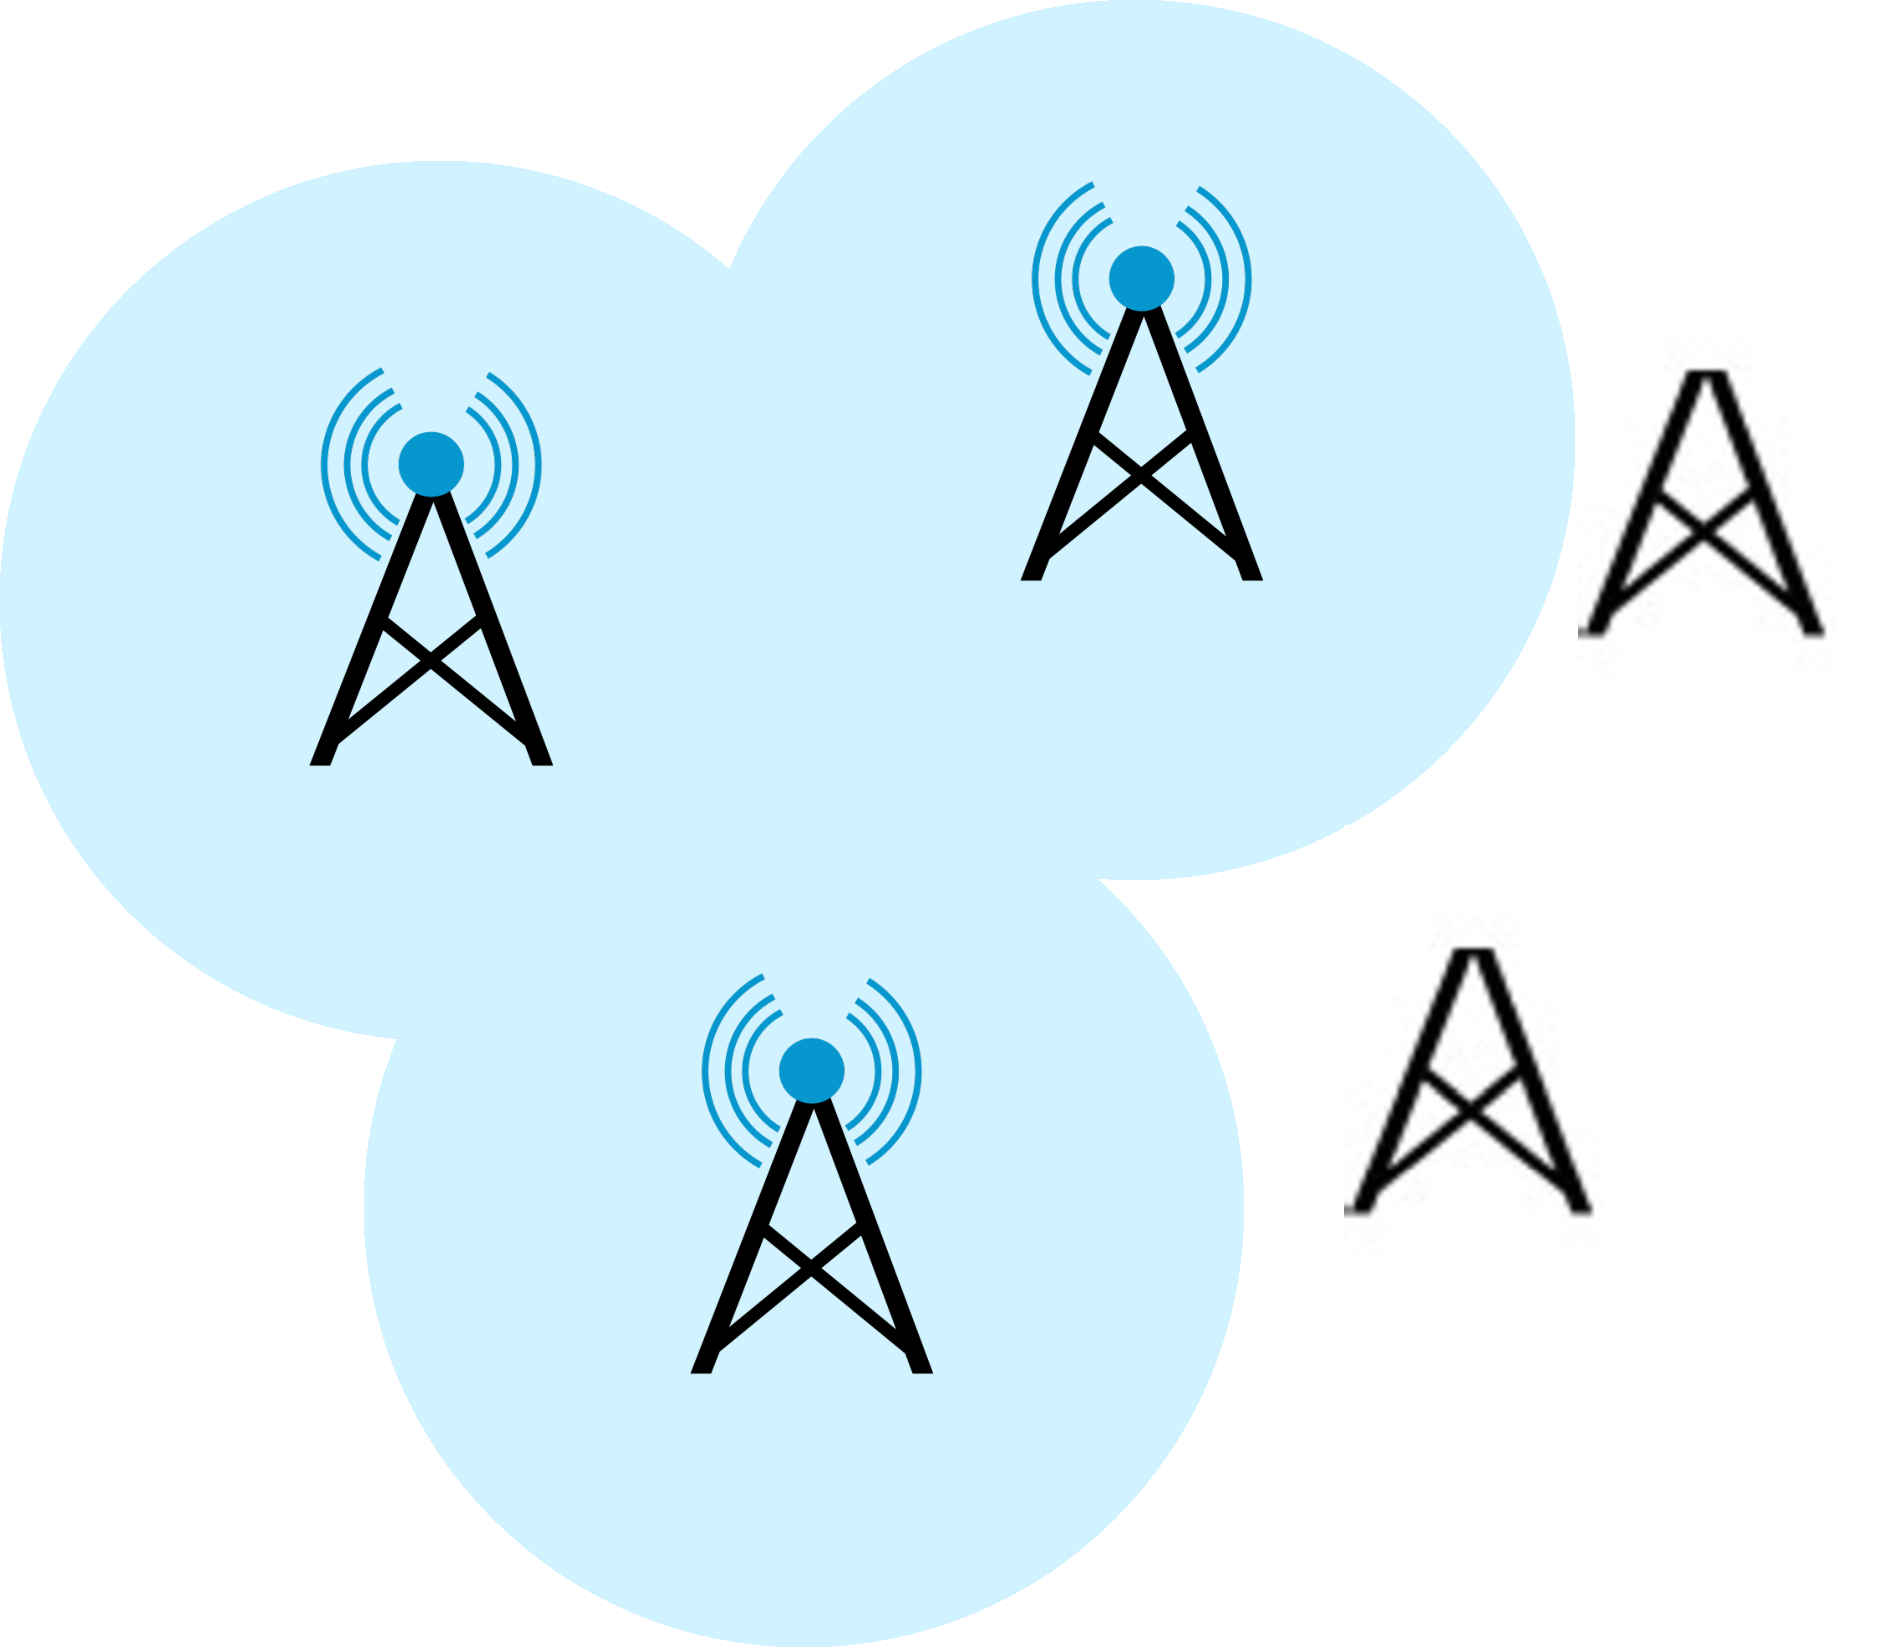
\includegraphics[width=\linewidth]{figs/coverage.pdf}
    \end{column}
    \end{columns}
\end{frame}


\begin{frame}{例: 不可分財の分配}

    \begin{columns}
    \begin{column}{.55\textwidth}
    $U = \{v_1, \dots, v_n\}$ ... 財の集合 \\
    $f_i$ ... $i$さんの効用関数，単調劣モ ($i=1,\dots, m$)
    \begin{block}{}
        \alert{社会効用}$\sum_{i=1}^m f_i(X_i)$が最大の分配$(X_1, \dots, X_m)$を求めたい．
    \end{block}
    \end{column}
    \begin{column}{.4\textwidth}
    \begin{tikzpicture}[>=latex]
        \foreach \i/\emoji in {1/👦,2/🐶,3/🐱} {
            \node[inner sep=0pt, "{$f_\i$}" left](v\i) at ($(0, -\i*2)$) {\coloremoji[scale=2]{\emoji}};
        }
        \foreach \j/\emoji in {1/🍙,2/🍜,3/🍖,4/🐟} {
            \node[inner sep=0pt](w\j) at ($(4, -\j*1.6)$) {\coloremoji[scale=2]{\emoji}};
        }
        \graph[edges={thick, UniBlue}]{
            (v1) <- {(w1), (w2)};
            (v2) <- (w3);
            (v3) <- (w4);
        };
    \end{tikzpicture}
    \end{column}
    \end{columns}
\end{frame}

\begin{frame}{例: 不可分財の分配}

    \begin{columns}[T]
    \begin{column}{.55\textwidth}
        \begin{itemize}
        \item $V := U$の$m$個のコピー
        \item $f(X) := \sum_{i=1}^m f_i(X \cap U_i)$
        \item $\caC$: $V$上の分割マトロイド（各財は1人まで割当可能）
        \end{itemize}
        \vspace{1em}
        \bf 分割マトロイド制約の単調劣モ最大化
    \end{column}
    \begin{column}{.4\textwidth}
    \begin{tikzpicture}[>=latex]
        \foreach \i/\emoji in {1/👦,2/🐶,3/🐱} {
            \node[inner sep=0pt, "{$U_\i$}" left](v\i) at ($(0, -\i*1.5)$) {\coloremoji[scale=1.5]{\emoji}};
            \node[inner sep=0pt](item\i1) at ($(1, -\i*1.5)$) {\coloremoji[scale=1.5]{🍙}};
            \node[inner sep=0pt](item\i2) at ($(2, -\i*1.5)$) {\coloremoji[scale=1.5]{🍜}};
            \node[inner sep=0pt](item\i3) at ($(3, -\i*1.5)$) {\coloremoji[scale=1.5]{🍖}};
            \node[inner sep=0pt](item\i4) at ($(4, -\i*1.5)$) {\coloremoji[scale=1.5]{🐟}};
        }
        \draw (.5, -1.0) -- (.5, -5) -- (4.5, -5) -- (4.5, -1.0) -- cycle;
        \draw[dotted, thick] (1.5, -1.0) -- (1.5, -5);
        \draw[dotted, thick] (2.5, -1.0) -- (2.5, -5);
        \draw[dotted, thick] (3.5, -1.0) -- (3.5, -5);
    \end{tikzpicture}
    \end{column}
    \end{columns}
\end{frame}


\begin{frame}{例: 文書要約~\cite{Lin2011}}
    \small
    \begin{columns}
        \begin{column}{.6\linewidth}
    $V$: 元文書の文全ての集合, $X \subseteq V \longleftrightarrow$ 要約  \\
    $r_1, \dots, r_K$: 参照文 \\
    $c_e(X) = $ n-gram $e$ が要約$X$に現れる回数 \\
    $M_{e,i} =$ n-gram $e$ が参照文 $r_i$に現れる回数

    \begin{block}{ROUGE-N}
        \[
        f(X) = \sum_{r \in R}\sum_{e: \text{文$r$に含まれるn-gram}} \min\{ c_e(X), M_{e,i} \}
        \]
        {\footnotesize (※ 簡単のため正規化定数は省いた)}
    \end{block}
        \end{column}
        \begin{column}{.3\linewidth}
            \footnotesize
            \begin{tcolorbox}[title=要約文,colback=white,sharp corners]
            \highlight{民間英語試験}の延期を決定した．
            \end{tcolorbox}

            \begin{tcolorbox}[title=参照文A,colback=white,sharp corners]
            英語教育が専門の〇〇氏は，\highlight{民間英語試験}は問題が多く，...
            \end{tcolorbox}
        \end{column}
    \end{columns}

    \begin{itemize}
        \item ROUGE-Nは単調劣モジュラ関数
        \item サイズ制約$\longleftrightarrow$ 要約に使える文の数に制約
        \item ナップサック制約 $\longleftrightarrow$ 要約の文字数に制約
    \end{itemize}
\end{frame}

\begin{frame}{例: モデル解釈(SP-LIME)~\cite{Ribeiro2016}}
    近年の機械学習モデルは複雑で解釈しづらい．→\textbf{解釈性}

    \vspace{1em}
    \structure{Local Iterpretable Model-agnostic Explanations (LIME)} \\
    各訓練データに対して，“特徴量ごとの予測への貢献度”を計算してくれる手法
    \begin{center}
        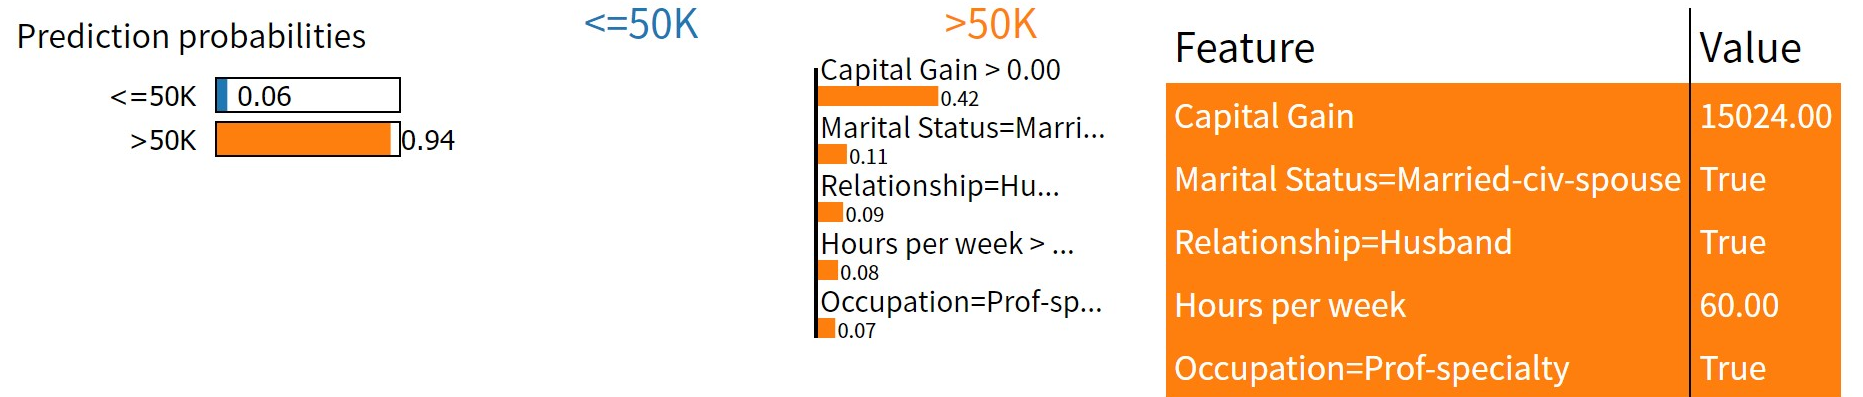
\includegraphics[height=2.5cm]{figs/LIME.png}\\
        {\tiny\hfill 引用: LIMEのチュートリアル}
    \end{center}

    \vfill
    \begin{center}
        \bf データセット全体での挙動を知りたい場合は？
    \end{center}

\end{frame}

\begin{frame}{例: モデル解釈(SP-LIME)~\cite{Ribeiro2016}}
    \small
    \begin{columns}
        \begin{column}{.65\textwidth}
    $V = $ 訓練データの集合 \\
    $U = $ 特徴量の集合 \\
    $a_{ij} = $  データ$i$に対する特徴量$j$のLIMEスコア \\
    $G = (V, U; E)$ ... $a_{ij}>0$の$(i,j)$に枝を引いた二部グラフ \\
    $w_j := \sqrt{\sum_{i \in V} a_{ij}}$ ... 特徴量$j$の重み
        \end{column}
        \begin{column}{.3\textwidth}
            \begin{tikzpicture}
                \graph[mygraph, grow right=4em]{
                    subgraph I_nm[V={1,2,3,4}, W={a,b,c,d}];
                    1 -- {a, b};
                    2 -- {b, c};
                    3 -- {c};
                    4 -- {a, d};
                };
                \begin{scope}[on background layer]
                    \node[draw,UniBlue,fill=UniBlue!10,rectangle,dotted,thick,fit=(1) (2),"$X$" {UniBlue,left}]{};
                    \node[draw,AlertOrange,fill=AlertOrange!10,rectangle,dotted,thick,fit=(a) (b) (c),"$\Gamma(X)$" {AlertOrange,right}]{};
                \end{scope}
            \end{tikzpicture}
        \end{column}
    \end{columns}

    \begin{block}{}
        \[
        f(X) = \sum_{j \in \Gamma_G(X)} w_j
        \]
    \end{block}
    \begin{itemize}
        \item モデルの全体的挙動を理解する上で多様な訓練データを抽出できる
        \item サイズ制約 $\longleftrightarrow$ 抽出するデータ数に制約
    \end{itemize}
\end{frame}

\begin{frame}{例: 変数選択~\cite{Das2011,Elenberg2018}}
    $V = \{1, \dots, n\}$ \\
    $\bx_i$: 説明変数 ($i = 1,\dots, n$), $\by$: 被説明変数

    \begin{block}{}
        \[
        f(X) = \norm{\by}_2^2 - \min_{\beta:\supp(\beta) \subseteq X} \norm*{ \by - \sum_{i=1}^n \beta_i \bx_i }_2^2
        \]
    \end{block}
    \hfill ... $X$に入っている変数だけ使ったときの最良残差

    \vfill
    \begin{itemize}
        \item 抑圧変数がない $\implies$ $f$: 単調劣モジュラ
        \item $X = [\bx_1 \dots \bx_n]$ に対するRIP仮定 $\implies$ $f$: 弱劣モジュラ（近似的に劣モジュラ）
    \end{itemize}
\end{frame}

%%%%%%%%%%%%%%%%%%%%%%%%%%%%%%%%%%
\section{アルゴリズム}
\againframe<3>{outline}
%%%%%%%%%%%%%%%%%%%%%%%%%%%%%%%%%%

\begin{frame}<1-2>[label=algorithms]
    \frametitle{最大化アルゴリズム}

    \structure{サイズ制約$\abs{X} \leq k$（組合せ的アルゴリズム）}
    \begin{itemize}
        \item \alert<2>{古典貪欲法}~\cite{Nemhauser1978}
        \item \alert<2>{確率的貪欲法}~\cite{Mirzasoleiman2015}
    \end{itemize}

    \vfill
    \structure{一般の制約$X \in \caC$（連続最適化的アルゴリズム）}
    \begin{itemize}
        \item \alert<3>{連続貪欲法}~\cite{Calinescu2011,Chekuri2010,Vondrak2014}
    \end{itemize}
\end{frame}

\begin{frame}<1-2>[label=greedy]{古典貪欲法~\cite{Nemhauser1978}}
    \small
    \begin{block}{}
        \begin{algorithmic}[1]
            \STATE $X_0 \gets \emptyset$
            \FOR{$i = 1, \dots, k$}
            \STATE $a \in V \setminus X_{i-1}$ のうち$f(X_{i-1} \cup a)$ が最大のものを
            求め，$a_i$とする．
            \STATE $X_i \gets X_{i-1} \cup a_i$
            \ENDFOR %
            \RETURN $X=X_k$
        \end{algorithmic}
    \end{block}
    \vfill
    \begin{itemize}
        \item<2-> 貪欲アルゴリズムの出力を$X$とすると，
        \[
            f(X) \geq (1-1/e) \highlightcap{$\displaystyle\max_{X^*: \abs{X^*}=k} f(X^*)$}{最適値}
        \]
        \item<3-> $O(nk)$回の$f$の関数値評価が必要 ($n=|V|$, $k$:サイズ制約) \\
        → \alert{応用によっては重すぎる}
    \end{itemize}
\end{frame}

\begin{frame}
    \frametitle{古典貪欲法の解析}
    \footnotesize
    \begin{columns}[T]
    \begin{column}{.5\textwidth}
    \setlength{\abovedisplayskip}{0pt}
    \begin{lemma}
        $f$: 劣モジュラ
        \[
            f(X \cup Y) \leq f(X) + \sum_{a \in Y \setminus X} [f(X \cup a) - f(X)]
        \]
    \end{lemma}
    \onslide<2->{
    \begin{lemma}
        各$i=1,2,\dots,k$に対して
        \[
            f(X_i) - f(X_{i-1}) \geq \frac{1}{k} [f(X^*) - f(X_{i-1})]
        \]
    \end{lemma}
    {\hfill\scriptsize $X^*$: 最適解}
    }
    \begin{lemma}<3->
        各$i=0,1,2,\dots,k$に対して
        \[
            f(X^*) - f(X_i) \leq \left(1 - \frac{1}{k}\right)^i f(X^*)
        \]
    \end{lemma}
    \end{column}
    \begin{column}{.47\textwidth}
        \begin{alertblock}<4->{定理}
        \[
            f(X_k) \geq (1-1/e) f(X^*)
        \]
        \end{alertblock}
    \end{column}
    \end{columns}
    \onslide<2>
    \postit{
        $X_0 = \emptyset$ \\
        $X_i = X_{i-1} \cup a_i$ \\
        $a_i \in \argmax_{a \in V \setminus X_{i-1}} f(X_{i-1} \cup a)$
        }
\end{frame}

\againframe<3->{greedy}

\begin{frame}{確率的貪欲法~\cite{Mirzasoleiman2015}}
    $\epsilon >0$ を固定．
    \begin{block}{}
    \begin{algorithmic}[1]
        \STATE $X_0 \gets \emptyset$
        \FOR{$i=1, \dots, k$}
        \STATE $R_i:= V\setminus X_{i-1}$ から$\frac{n}{k}\log\frac{1}{\epsilon}$ 個ランダムサンプル
        \STATE $a_i \in \argmax_{a \in R_i} f(X_{i-1}\cup a)$
        \STATE $X_{i} \gets X_{i-1} \cup a_i$
        \ENDFOR
        \RETURN $X=X_k$
    \end{algorithmic}
    \end{block}

    \pause
    \begin{itemize}
        \item
        $
            \E [ f(X)] \geq (1-1/e-\epsilon) f(X^*)
            $
        \item $O(n\log(1/\epsilon))$回の関数値評価 \\
        \alert{古典貪欲法の$O(nk)$に比べて改善！}
    \end{itemize}
\end{frame}

\againframe<3>{algorithms}

\begin{frame}<1-4>[label=contgreedy]{連続貪欲法~\cite{Calinescu2011}}
    % \small
    \begin{center}
    \begin{tikzpicture}[>=latex]
        \tikzset{block/.style={fill=cyan!10,rectangle,rounded corners,align=center}};
        \tikzset{myarrow/.style={draw=black!50,ultra thick}};
        \node[block](v1){\textcolor{UniBlue!70!black}{\bf 元問題}\\ $\max\left\{f(X) : X \in \caC \right\}$ };
        %
        \onslide<2->
        \node[block,fill=AlertOrange!20,right=3cm of v1](v2){\textcolor{AlertOrange}{\bf 緩和問題} \\ $\max\left\{F(\bx) : \bx \in P \right\}$ };
        \draw[myarrow, ->] (v1) -- node[above]{\alert<5>{①連続緩和}} (v2);
        %
        \onslide<3->
        \node[block,fill=AlertOrange!20,below=2.5cm of v2](v3){ $\bx \in P$ \\ s.t. \\ $F(\bx) \geq (1-1/e) f(X^*)$};
        \node[below=1pt of v3]{\footnotesize $X^*$:最適解};
        \draw[myarrow, ->] (v2) -- node[right,align=left]{\alert<6>{②連続貪欲法}} (v3);
        %
        \onslide<4->
        \node[block] at (v1 |- v3) (v4){$X \in \caC$ \\ s.t. \\ $f(X) \geq (1-1/e) f(X^*)$};
        \draw[myarrow, ->] (v3) -- node[below]{\alert<7>{③丸め}} (v4);
    \end{tikzpicture}
    \end{center}
\end{frame}


\againframe<5|handout:0>{contgreedy}

% \begin{frame}{集合から$\{0,1\}$ベクトルへ}
%     \begin{columns}
%         \begin{column}{.6\linewidth}
%     % \small
%     集合 $X \subseteq V$ と ベクトル$\bfone_X \in \{0,1\}^n$ を対応させる. ($n=|V|$)
%     \[
%         (\bfone_X)_i = \begin{cases}
%             1 & i \in X \\
%             0 & i \not\in X
%         \end{cases}
%     \]
%         \end{column}
%         \begin{column}{.4\linewidth}
%             \tikzset{vertex/.style={fill=black,circle,inner sep=2pt}}
%            \begin{tikzpicture}[>=latex,scale=.15em]
%             \draw[->] (0,0) -- (0,1.5);
%             \draw[->] (0,0) -- (1.5,0);
%             \foreach \x\y in {0/0,0/1,1/0,1,1}
%                 \node[vertex](\x\y) at (\x,\y) {};
%             \draw[dotted] (01) -- (11) -- (10) ;
%             \node[below=.1em of 00] {$\emptyset$};
%             \node[below=.1em of 10] {$\{1\}$};
%             \node[left=.1em of 01] {$\{2\}$};
%             \node[above=.1em of 11] {$\{1,2\}$};
%            \end{tikzpicture}
%         \end{column}
%     \end{columns}

%     \vfill
%     集合関数 $f:2^V\to\R$ は $\{0,1\}^n$上の関数とみなせる.
% \end{frame}

\tikzset{blackvertex/.style={fill=black,circle,inner sep=2pt}}
\tikzset{orangevertex/.style={fill=AlertOrange,circle,inner sep=2pt}}

% \begin{frame}{実行可能領域: 集合族の凸包}
%     \begin{columns}
% \begin{column}{.6\linewidth}
%     集合族 $\caC \subseteq 2^V$ の\alert{凸包} $P$ を
%     \[
%       P = \conv\{ \bfone_X : X \in \caC \}
%     \]
%     と定める.
% \end{column}
% \begin{column}{.4\linewidth}
%            \begin{tikzpicture}[>=latex,scale=.15em]
%             \draw[fill=AlertOrange!10] (0,0) -- (1,0) -- (0,1) -- cycle;
%             \draw[->] (0,0) -- (0,1.5);
%             \draw[->] (0,0) -- (1.5,0);
%             \foreach \x\y in {0/0,0/1,1/0}
%                 \node[orangevertex](\x\y) at (\x,\y) {};

%             \node[blackvertex] (11) at (1,1) {};
%             \draw[dotted] (01) -- (11) -- (10);
%            \end{tikzpicture}
% \end{column}
%     \end{columns}

%     \vfill

%     \begin{itemize}
%         \item $P$上の線形最適化は容易であることが多い (e.g., マトロイド制約: 貪欲法)
%         \item $X \in \caC$に対し $\forall Y \subseteq X$ も$Y\in\caC$\\
%         $\implies$ $\bx \in P$ に対し $\bfzero \leq \forall \by \leq \bx$も$\by \in P$ (\alert{down closed})
%     \end{itemize}
% \end{frame}

\begin{frame}{多重線形拡張(multilinear extension)}
    % \small
    % 集合関数をそれっぽく連続関数に拡張したもの
    \begin{block}{}
        $f$の\alert{多重線形拡張} $F:[0,1]^n \to \R$
    \begin{align*}
    F(\bx) &:= \sum_{S \subseteq V} f(S) \prod_{i \in S} x_i \prod_{i \not\in S} (1-x_i) \\
        &= \E [ f(R(\bx)) ]
    \end{align*}
    $R(\bx)$: 要素$i$を確率$x_i$で独立に含むランダム集合
    \end{block}

    \vfill
    \structure{注} $F$, $\nabla F$ は任意の精度で近似的に求められる(サンプリング)．\\
    以下，簡単のため $F$, $\nabla F$ を与えるオラクルがあるものとする．
\end{frame}

\begin{frame}{多重線形拡張(multilinear extension)}
    % \small
    \begin{columns}
        \begin{column}{.5\textwidth}
    \structure{性質}
    \begin{itemize}
        \item $F(\bfone_X) = f(X)$
        \item $f$:単調 $\implies \nabla F \geq \bfzero$
        \item $f$:劣モ $\implies \frac{\partial^2 F}{\partial x_i \partial x_j} \leq 0$ ($i \neq j$) \\
        特に$F$は非負方向に凹, \\
        $\be_i - \be_j$ 方向に凸
        \end{itemize}
    \end{column}
        \begin{column}{.5\textwidth}
        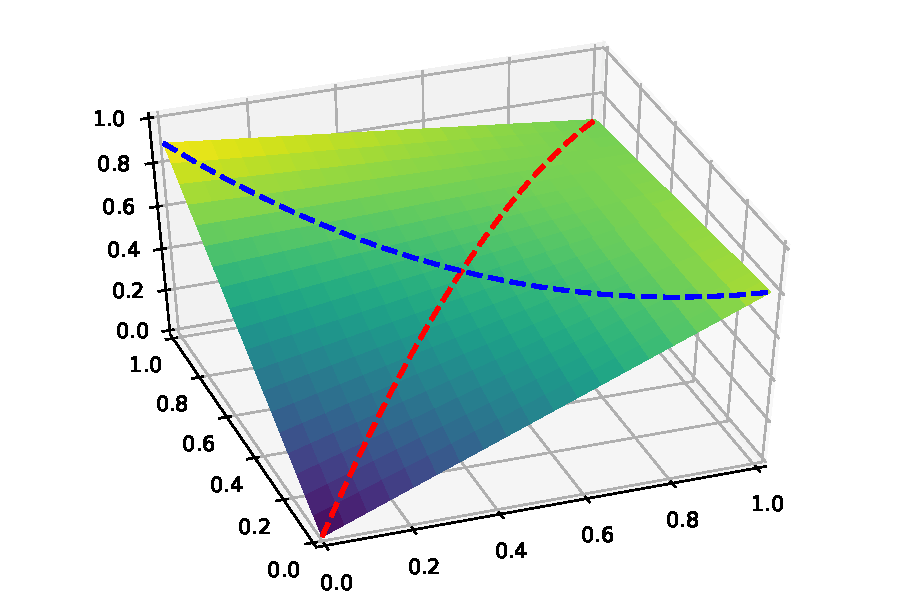
\includegraphics[width=\linewidth]{figs/MLext.pdf}
    \end{column}
    \end{columns}
    ※一般には\alert{凸でも凹でもない}
\end{frame}

\begin{frame}[t]{多重線型拡張の性質}
    \small
    \begin{lemma}
        $f$:単調 $\implies \nabla F \geq \bfzero$
    \end{lemma}

        $i \in V$を任意に取る．$\nabla F(\bx)_i$を計算してみると
        \[
            \nabla F(\bx)_i = \sum_{X \subseteq V \setminus i} f(X \cup i)\Pr(X) - \sum_{X \subseteq V \setminus i} f(X)\Pr(X).
        \]
        ここで，$\Pr(X) = \prod_{k \in X}x_k \prod_{k \notin X: k \neq i} (1 - x_k)$である．
        $f$の単調性より$f(X \cup i) - f(X) \geq 0$なので，$\nabla F(\bx)_i \geq 0$.
\end{frame}

\begin{frame}[t]{多重線型拡張の性質}
    \small
    \begin{lemma}
        $f$:劣モ $\implies \frac{\partial^2 F}{\partial x_i \partial x_j} \leq 0$ ($i \neq j$) \\
        特に$\varphi(t) = F(\bx + t \boldsymbol{d})$ ($\boldsymbol{d}\geq \zeros$) は凹関数，
        $\psi(t) = F(\bx + t(\be_i - \be_j))$は凸関数
    \end{lemma}

        $i = j$の場合は自明に$\frac{\partial^2 F}{\partial x_i \partial x_j} = 0$. $i\neq j$のとき，
        \[
            \frac{\partial^2 F}{\partial x_i \partial x_j}(\bx) =
            \sum_{X \subseteq V\setminus\{i, j\}}
            [f(X \cup i \cup j) + f(X) - f(X \cup i) - f(X \cup j)]\Pr(X).
        \]
        ここで，$\Pr(X) = \prod_{k \in X}x_k \prod_{k \notin X: k \neq i, j} (1 - x_k)$である．
        劣モジュラ性より$f(X \cup i \cup j) + f(X) - f(X \cup i) - f(X \cup j) \leq 0$なので$\frac{\partial^2 F}{\partial x_i \partial x_j}(\bx)\leq 0$.
\end{frame}

\begin{frame}[t]{多重線型拡張の性質}
    \small
    \begin{lemma}
        $f$:劣モ $\implies \frac{\partial^2 F}{\partial x_i \partial x_j} \leq 0$ ($i \neq j$) \\
        特に$\varphi(t) = F(\bx + t \bv)$ ($\bv \geq \zeros$) は凹関数，
        $\psi(t) = F(\bx + t(\be_i - \be_j))$は凸関数
    \end{lemma}

    連鎖律より
    \[
        \varphi''(t) = \sum_{i, j \in V} \frac{\partial^2 F}{\partial x_i \partial x_j}(\bx+t\bv) v_iv_j
    \]
    であるが，$\frac{\partial^2 F}{\partial x_i \partial x_j}(\bx+t\bv) \leq 0$で，仮定より$v_i, v_j \geq 0$であるから，
    $\varphi''(t) \leq 0$.
    よって$\varphi$は凹関数．

    \pause
    \bigskip
    再び連鎖律より
    \[
        \psi''(t) = -2\frac{\partial^2 F}{\partial x_i \partial x_j}(\bx+t(\be_i-\be_j)) \geq 0
    \]
\end{frame}

\againframe<6|handout:0>{contgreedy}

\begin{frame}{連続貪欲法(連続時間版)}
    \small
    \begin{block}{連続緩和問題}
        \setlength{\abovedisplayskip}{0pt}
        \begin{align*}
            \max \quad F(\bx) \quad \text{s.t.} \quad \bx\in P
        \end{align*}
    \end{block}

    \onslide<2->
    \begin{columns}[T]
        \begin{column}{0.6\paperwidth}
            以下の微分方程式に従って$\bx(t)$を動かす
            \begin{block}{}
            \setlength{\abovedisplayskip}{0pt}
            \setlength{\belowdisplayskip}{0pt}
            \begin{align*}
                \bx(0) &= \bfzero \\
                \frac{d\bx(t)}{dt} &= \argmax_{\bv \in P} \nabla F(\bx(t))^\top \bv
            \end{align*}
            \end{block}
            \vfill
            \onslide<3->{
\begin{theorem}[\cite{Calinescu2011}]
    $f$: 単調劣モ, $P$: down closed \\
    $\implies \bx(1)\in P$ かつ $F(\bx(1)) \geq (1-1/e) \max_{\bx^* \in P} F(\bx^*)$
\end{theorem}
            }
        \end{column}
        \begin{column}{0.3\paperwidth}
            % \includegraphics[width=.6\linewidth]{figs/contgreedy.pdf}
            \begin{tikzpicture}[>=latex,scale=.35em]
            \draw[->] (0,0) -- (0,1.1);
            \draw[->] (0,0) -- (1.1,0);
            \draw[fill=AlertOrange!10] (0,1) -- (1,0) -- (0,0) -- cycle;
            \node[below] at (0,0) {$\bx(0)$};
            \coordinate (x1) at (0.5,0.5);
            \node[right=1pt of x1] {$\bx(1)$};
            \draw[ultra thick,UniBlue] (0,0) .. controls (.2,0) and (.3, .5)  .. (x1)
                coordinate[pos=0.4] (xt) node[right=3pt of xt]{$\bx(t)$};
            \node[blackvertex] at (xt) {};
            \draw[ultra thick,->,AlertOrange] (xt) -- ++($0.5*(.3,.5)$) node[pos=.9,left]{$\bv(t)$};
        \end{tikzpicture}
        \end{column}
    \end{columns}
\end{frame}

\begin{frame}{解析}
    \small
$\Psi(t) := e^{t-1}F(\bx(t))$ とする.
$\frac{d\Psi}{dt} = e^{t-1}[F(\bx(t)) + \nabla F(\bx(t))^\top \frac{d\bx(t)}{dt}]$.

\vfill
$\bx^* \in P$ を最適解,  $\bx^* \vee \bx(t)$ を $\bx^*$と$\bx(t)$の成分ごとにmaxをとったベクトルとする.

\begin{columns}
    \begin{column}{.7\linewidth}
\begin{align*}
    F(\bx^*)
    &\leq F(\bx^* \vee \bx(t)) \\
    &\leq F(\bx(t)) + \nabla F(\bx(t))^\top (\bx^* \vee \bx(t) - \bx(t)) \\
    &\leq F(\bx(t)) + \nabla F(\bx(t))^\top \bv(t) \\
    &= F(\bx(t)) + \nabla F(\bx(t))^\top \dfrac{d\bx(t)}{dt}
\end{align*}
    \end{column}
    \begin{column}{.3\linewidth}
        \begin{tikzpicture}[>=latex,scale=.3em]
            \draw[fill=AlertOrange!10] (0,0) -- (1,0) -- (0,1) -- cycle;
            \node[blackvertex,"$\bx(t)$" below](xt) at (.5,.3) {};
            \node[blackvertex,"$\bx^*$" above] (xs) at (0,1) {};
            \node[blackvertex,"$\bx(t)\vee\bx^*$" above] (vee) at (xs -| xt) {};
            \draw[dotted] (xs) -- (vee);
            \draw[dotted, thick, AlertOrange] (xt) edge node[right]{\scriptsize この上で凹} (vee);
           \end{tikzpicture}
    \end{column}
\end{columns}

∴ $\frac{d\Psi}{dt} \geq e^{t-1}F(\bx^*)$.

\vfill
$[0,1]$で積分: $\Psi(1)-\Psi(0) = F(\bx(1)) \geq (1-e^{-1})F(\bx^*)$.
\end{frame}

\begin{frame}{連続貪欲法(離散時間版)}
    % \small
    実際には微分方程式を厳密に解くことはできないので，時間を離散化して近似する

    \begin{block}{}
    \begin{algorithmic}[1]
        \STATE $\bx(0) = \bfzero$
        \FOR{$t=0,\delta,2\delta, \dots, 1-\delta$}
            \STATE $\bv(t) \in  \argmax_{\bv \in P} \nabla F(\bx(t))^\top \bv$ を求める
            \STATE $\bx(t+\delta) \gets \bx(t) + \delta \bv(t)$
        \ENDFOR
        \RETURN $\bx(1)$
    \end{algorithmic}
    \end{block}

    \begin{itemize}
        \item Frank-Wolfe法の亜種
        \item 精度$\epsilon>0$に応じて 時間幅$\delta$を十分小さく取れば，同様の仮定のもと $F(\bx) \geq (1-1/e-\epsilon) \max_{\bx^* \in P}F(\bx^*)$
    \end{itemize}
\end{frame}

\againframe<7|handout:0>{contgreedy}

\begin{frame}{丸めアルゴリズム}
    連続貪欲法で得られる緩和解$\bx$は$\{0,1\}$ベクトルとは限らないので，$\{0,1\}$ベクトルに丸める必要がある.

    →\alert{制約ごとに丸めアルゴリズムを設計}

    \vfill
    \textbf{マトロイド制約}
    \begin{itemize}
        \item Pipage Rounding~\cite{Calinescu2011}
        \item Swap Rounding~\cite{Chekuri2010}
    \end{itemize}

    \textbf{その他の制約}
    \begin{itemize}
        \item Contention Resolution Scheme~\cite{Vondrak2014}
    \end{itemize}
\end{frame}

\begin{frame}{Pipage Rounding~\cite{Calinescu2011}}
    \small
    \begin{columns}
        \begin{column}{.65\linewidth}
    \begin{enumerate}
        \item $x_i, x_j$ が\{0,1\} でない$i, j \in V$を取る
        \item $\alpha_+ = \max\{\alpha \geq 0 : \bx + \alpha(\be_i - \be_j) \in P \}$ \\
         $\alpha_- = \max\{\alpha \geq 0 : \bx - \alpha(\be_i - \be_j) \in P \}$
        \item $\bx_+ = \bx + \alpha_+(\be_i-\be_j)$, $\bx_- = \bx - \alpha_-(\be_i-\be_j)$ のうち $F$ の値が大きいものに $\bx$を更新
        \item $P$をぶつかった面に制限して 1に戻る
    \end{enumerate}
        \end{column}
        \begin{column}{.3\linewidth}
            \pgfmathsetmacro{\radi}{1.8}
            \begin{tikzpicture}[>=latex]
                \draw [fill=AlertOrange!10] (0:\radi) -- (60:\radi) -- (120:\radi) -- (180:\radi) -- (240:\radi) -- (300:\radi) -- cycle;
                \node[blackvertex, "$\bx$" below] (x) at (0.2,0.1) {};
                \node[blackvertex, "$\bx_+$" above] (xp) at ($(120:\radi)!(x)!(180:\radi)$) {};
                \node[blackvertex, "$\bx_-$" right] (xm) at ($(300:\radi)!(x)!(0:\radi)$) {};
                \draw[->] (x) edge node[midway,below]{$\alpha_+$} (xp);
                \draw[->] (x) edge node[midway,below]{$\alpha_-$} (xm);
            \end{tikzpicture}
        \end{column}
    \end{columns}

    \begin{theorem}
        $P$: マトロイド多面体のとき，Pipage Roundingの出力$\overline{\bx}$は$\{0,1\}$ベクトルで，
        $F(\overline{\bx}) \geq F(\bx)$を満たす（$\bx$: Pipage Roundingの初期点）
    \end{theorem}
\end{frame}

\begin{frame}
    \frametitle{劣モジュラ最大化: 発展的な話題}
    \small

    \begin{columns}
        \begin{column}{.5\linewidth}
    \structure{整数格子点上の劣モジュラ最大化}
    \begin{itemize}
        \item 最適予算配分問題
        \item 最大化アルゴリズム
    \end{itemize}

    \vfill
    \structure{連続劣モジュラ関数}
    \begin{itemize}
        \item 非凸連続最適化（\alert{連続DR劣モジュラ関数}）
    \end{itemize}

    \structure{オンライン劣モジュラ最大化}
    \begin{itemize}
        \item 近似no-regretアルゴリズム
        \item 連続DR劣モジュラ関数のCVaR最大化
    \end{itemize}
        \end{column}
        \begin{column}{.4\linewidth}
\begin{tikzpicture}[>=latex, node distance = 2cm,scale=.6]
		\fill[orange!30] (0,0) -- (0,4) -- (4,0) -- (0,0);
		\draw[orange!70, line width=2pt, dotted] (0, 4) -- (4,0);
        \draw[->] (-0.5,0)--(5.5,0);
        \draw[->] (0,-0.5)--(0,4.5);
       \foreach \x in {0,1,2,3,4}
		\foreach \y in {0,1,2,3}
		{
			\fill (\x,\y) circle (3pt);
		}
\end{tikzpicture}

        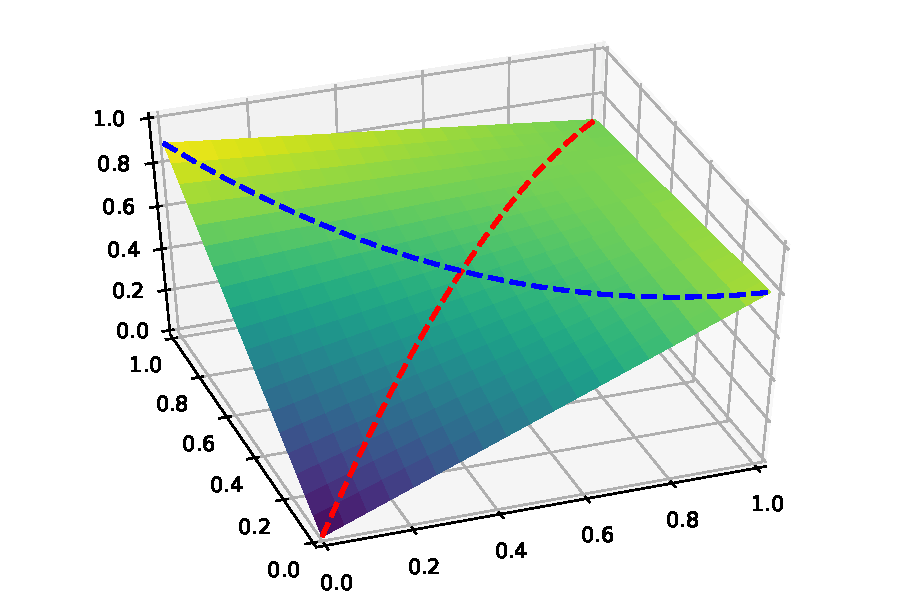
\includegraphics[width=\linewidth]{figs/MLext.pdf}
        \end{column}
    \end{columns}
\end{frame}

\section{まとめ}
\begin{frame}[allowframebreaks]{}
    \structure{参考文献}
    \renewcommand*{\bibfont}{\scriptsize}
    \printbibliography
\end{frame}
\end{document}